\chapter[Análise dos Resultados]{Análise dos Resultados}

Este capítulo tem como objetivo discutir os cenários de teste utilizados durante a pesquisa, assim como os resultados obtidos durante a realização da mesma.
Dentre estes resultados, estão presentes as fontes de erros levantadas com a experiência da pesquisa, suas respectivas correções, dentro do possível, e a análise da
viabilidade da utilização do Filtro de Partículas no contexto simplificado da Robótica Educacional. Desse modo, este capítulo está dividido
em três seções: \ref{sec:cenarios_teste}, \ref{sec:fontes_de_erros} e \ref{sec:viabilidade}.

\section{Cenários de Teste}
\label{sec:cenarios_teste}
\chapter[Cenários de Teste]{Cenários de Teste}
\label{sec:cenarios_teste}
O principal objetivo dos cenários de teste é apoiar a observação e análise sistemática da técnica de auto-localização utilizada durante o trabalho, assim como as diferentes configurações do ambiente e
do filtro utilizado.

Após a realização de todos os cenários de teste propostos, deve-se chegar a uma conclusão referente a viabilidade da utilização da técnica do Filtro de Partículas em um contexto simplificado da robótica.

Os cenários de teste consistem em 10 situações onde a solução foi analisada, variando entre elas o ambiente e a configuração do filtro. Buscando
analisar a exatidão da auto-localização obtida em cada contexto, reiterando que o objetivo da pesquisa é analisar a viabilidade da utilização
de uma técnica de SLAM em um contexto simplificado.

O Filtro de Partículas é uma das duas principais técnicas que buscam solucionar o problema
de SLAM, por este motivo, os cenários de teste desta pesquisa buscam analisar o Filtro de Partículas sendo executado no contexto da Robótica
Educacional, o que viabilizaria, em parte, a aplicação da solução de SLAM no contexto simplificado.

Os dados obtidos a partir de cada cenário de teste está organizado de acordo com a Tabela \ref{tab:org_dados}.

\begin{table}[H]
  \centering
  \caption{Organização dos Dados}
  \label{tab:org_dados}
  \begin{tabular}{|c|c|c|c|c|c|}
  \hline
  \textbf{Exemplo} & \textbf{Partículas} & \textbf{Rotação} & \textbf{Deslocamento} & \textbf{Movimentos} & \textbf{Precisão} \\ \hline
  \end{tabular}
\end{table}

Onde,
\begin{itemize}
  \item \textbf{Exemplo} faz referência ao ciclo de teste. Cada cenário foi testado 5 (cinco) vezes, buscando obter a média como resultado
  final do cenário;

  \item \textbf{Partículas} informa a quantidade de partículas utilizada durante este teste;

  \item \textbf{Rotação} informa a velocidade de rotação do robô, em graus por segundo;

  \item \textbf{Deslocamento} informa a velocidade de deslocamento em linha reta, em centímetros por segundo;

  \item \textbf{Movimentos} apresenta o número de movimentos aleatórios que foram necessários para obtenção da localização;

  \item \textbf{Precisão} informando qual a precisão obtida no teste, classificada em \textit{Ótima}, \textit{Boa}, \textit{Mediana},
  \textit{Baixa} e \textit{Baixíssima}.
\end{itemize}

Durante os cenários de teste, o ambiente utilizado foi o apresentado na Figura \ref{img:map1}, onde todos os
valores se encontram em centímetros (cm).

\begin{figure}[H]
	\centering
	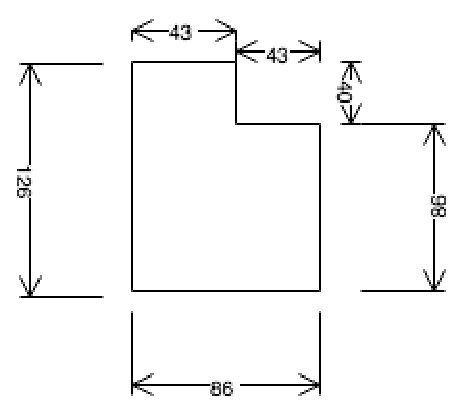
\includegraphics[scale=1.3]{figuras/map1.eps}
	\caption[Primeiro Cenário de Teste]{Mapa utilizado durante primeiro cenário de teste.}
	\label{img:map1}
\end{figure}

\subsection{Cenário de Teste 1}

Os resultados obtidos com o cenário estão dispostos na Tabela \ref{tab:cen1}. Deve-se atentar que o exemplo 3 possui um agravante, o
robô teve sua roda direita presa na parede enquanto se locomovia. Desse modo, o robô se perdeu e teve que se encontrar novamente, se comportando
da maneira esperada em um caso básico de "sequestro do robô".

Este cenário faz referência a variação da quantidade de partículas.

\begin{table}[H]
  \centering
  \caption{Resultados obtidos - Cenário 1}
  \label{tab:cen1}
  \begin{tabular}{|c|c|c|c|c|c|}
  \hline
  \textbf{Exemplo} & \textbf{Partículas} & \textbf{Rotação} & \textbf{Deslocamento} & \textbf{Movimentos} & \textbf{Precisão}\\ \hline
  1                & 200                   & 100             & 100                    & 9                & Ótima \\ \hline
  2                & 400                   & 100             & 100                    & 10                & Boa \\ \hline
  3                & 500                   & 100             & 100                    & 21                & Mediana \\ \hline
  4                & 100                   & 100             & 100                    & 5                & Mediana \\ \hline
  5                & 150                   & 100             & 100                    & 3                & Ótima \\ \hline
  \end{tabular}
\end{table}


\subsection{Cenário de Teste 2}

Os resultados obtidos com o cenário estão dispostos na Tabela \ref{tab:cen2}. Este cenário faz referência a variação da velocidade de
rotação do robô.

\begin{table}[H]
  \centering
  \caption{Resultados obtidos - Cenário 2}
  \label{tab:cen2}
  \begin{tabular}{|c|c|c|c|c|c|}
  \hline
  \textbf{Exemplo} & \textbf{Partículas} & \textbf{Rotação} & \textbf{Deslocamento} & \textbf{Movimentos} & \textbf{Precisão}\\ \hline
  1                & 150                   & 10             & 100                    & 7                & Boa \\ \hline
  2                & 150                   & 30             & 100                    & 6                & Ótima \\ \hline
  3                & 150                   & 50             & 100                    & 3                & Boa \\ \hline
  4                & 150                   & 70             & 100                    & 3                & Mediana \\ \hline
  5                & 150                   & 90             & 100                    & 8                & Mediana \\ \hline
  \end{tabular}
\end{table}


\subsection{Cenário de Teste 3}

Os resultados obtidos com o cenário estão dispostos na Tabela \ref{tab:cen2}. Este cenário faz referência a variação da velocidade de
deslocamento do robô, em unidades do diâmetro das rodas por segundo. Fixou-se a quantidade de partículas em 150, de acordo com os resultados
obtidos nos cenários anteriores, assim como a velocidade de rotação em 30 graus por segundo.

\begin{table}[H]
  \centering
  \caption{Resultados obtidos - Cenário 3}
  \label{tab:cen2}
  \begin{tabular}{|c|c|c|c|c|c|}
  \hline
  \textbf{Exemplo} & \textbf{Partículas} & \textbf{Rotação} & \textbf{Deslocamento} & \textbf{Movimentos} & \textbf{Precisão}\\ \hline
  1                & 150                   & 30             & 2                    & 4                & Baixa\\ \hline
  2                & 150                   & 30             & 5                    & 6                & Mediana\\ \hline
  3                & 150                   & 30             & 10                    & 3                & Baixa\\ \hline
  4                & 150                   & 30             & 15                    & 6                & Boa \\ \hline
  5                & 150                   & 30             & 30                    & 5                & Mediana\\ \hline
  \end{tabular}
\end{table}


\section{Fontes de Erros}
\label{sec:fontes_de_erros}

Como foi apresentado ao longo do trabalho, o mundo da robótica está envolto em erros. Desse modo, deve-se identificar o motivo do erro
para que o mesmo possa ser minimizado ao máximo, buscando garantir uma navegação adequada.
Por este motivo, durante a realização desta pesquisa, buscou-se identificar o maior número de fontes de erros possível para que as mesmas fossem
atacadas, minimizando a margem de erro durante o processo de auto-localização.

Cada fonte de erro identificada foi listada, com o objetivo de descrevê-la e apresentar uma possível solução que minimize o erro
advindo desta fonte. Esta listagem se encontra nas sub-seções \ref{sub:distancia_rodas}, \ref{sub:diametro}, \ref{sub:deslizes}, \ref{sub:precisao_sensores},
\ref{sub:caracteristica_sensor} e \ref{sub:colisao}.

\subsection{Distância entre Rodas}
\label{sub:distancia_rodas}

De acordo com o apresentado na seção \ref{sec:montagem_robo}, o robô utilizado é composto de duas rodas motorizadas que controlam
a movimentação do robô, e uma roda solta para apoio. Utilizando esta arquitetura de montagem, é possível realizar rotações sobre seu
próprio eixo, fazendo com que uma roda gire para frente e outra para tras. Esta técnica é utilizada a todo momento para movimentação
no ambiente, já que uma rotação sobre o próprio eixo possibilita o acompanhamento da direção em que o robô se locomove com maior clareza.

Utilizando a rotação sobre o próprio eixo, toda a navegação pode ser feita com base em cálculos trigonométricos, o que possibilita
a sua utilização no contexto educacional, seja no ensino superior, médio ou até fundamental. Desse modo, durante a realização desta pesquisa, busco-se
 a utilização de rotações sobre o próprio eixo para realização de curvas. A Figura \ref{img:rotacao_proprio_eixo} apresenta de forma
 clara o funcionamento da rotação.

 {\centering
 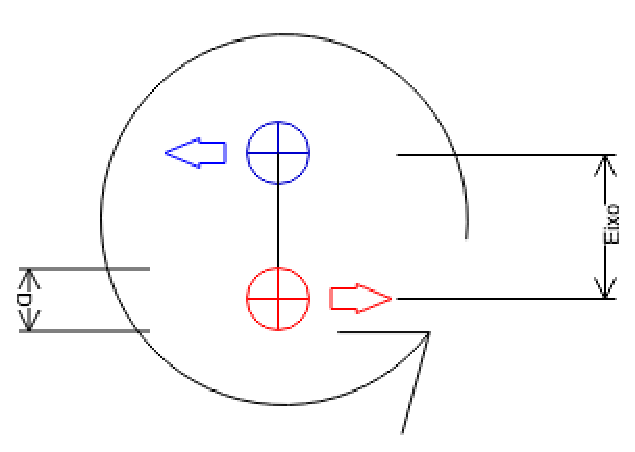
\includegraphics[scale=1.2]{figuras/rotacao_eixo.eps}
 \captionof{figure}{Rotação sobre o Próprio Eixo.}
 \label{img:rotacao_proprio_eixo}
 \par}

 Visto que que a solução utilizada envolve rotações sobre o próprio eixo, buscou-se minimizar ao máximo a margem de erro presente nesta
 técnica. Para que a rotação funcione da maneira desejada, deve-se conhecer, com o máximo de precisão, a distância entre cada roda,
 ou o eixo do robô (como pode ser observado na Figura \ref{img:rotacao_proprio_eixo}) e o diâmetro de cada roda, representado por "D" na
 Figura \ref{img:rotacao_proprio_eixo}.

 A distância entre cada roda é necessária pois quanto maior a distância, maior o número de giros em cada roda para que a mesma angulação
 seja alcançada. Dado que a distância entre cada roda é representada pela variável "eixo", o diâmetro de cada roda é representado pela
 variável "d" e a angulação, pela variável "a", a rotação é uma função que segue a assinatura \textit{f(a, eixo, d)}. Desse modo, cada um
 desses parâmetros é essencial para a garantia da precisão das rotações durante a movimentação do robô pelo mapa.

 A partir da experiência obtida durante a realização da pesquisa, pôde ser observado que a melhor forma de definir a distância entre as rodas
 e o diâmetro das mesmas, como descreve a seção \ref{sub:diametro}, é a definição por e calibração a partir de testes. Estas variáveis podem
 ser utilizadas como calibradores, que possibilitam a minimização de erros advindos de deslizes, como apresenta a seção \ref{sub:deslizes}.
 Desse modo, é possível esconder erros a partir da configuração destas variáveis. O sugerido é a configuração destas variáveis obervando
 resultados simples, como a realização de rotações completas e o erro final obtido.

\subsection{Diâmetro da Roda}
\label{sub:diametro}

  Assim como a comunidade de robótica mundial, esta pesquisa se baseia na utilização de sensores odométricos durante a navegação. Ou seja,
  as rotações de cada roda são registradas buscando calcular a distância e o sentido percorrido por cada roda. Esta informação possibilita
  que o robô saiba o quanto andou, para onde andou e, desse modo, possa concluir onde se encontra atualmente.

  A odometria se baseia na matemática básica, mais especificamente, na trigonometria. Possuindo a informação do tamanho de cada roda
  é possível saber a distância do pneu ao centro da roda, ou ponto de ligação ao eixo. Esta distância, ou raio da roda, possibilita o
   calculo da quantidade de rotação necessária para percorrer determinada distância por parte da roda. A Figura \ref{img:odometria_grafico}
   apresenta o fundamento da odometria, o que justifica a necessidade precisa do raio de cada roda.

   {\centering
   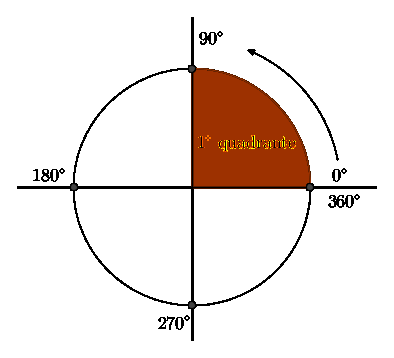
\includegraphics[scale=1]{figuras/odometria_grafico.eps}
   \captionof{figure}{Representação da Estratégia Odométrica.}
   \label{img:odometria_grafico}
   \par}

   A utilização da Odometria se baseia em um cálculo bastante simples, como apresenta a Figura \ref{img:odometria_grafico}. A distância percorrida
   na margem da circunferência destacada como primeiro quadrante faz referencia à distância percorrida pela roda em relação ao piso. A obtenção desta distância se torna fácil
   com o conhecimento do raio e da rotação feita pela roda.

   Deste modo, deve-se registrar o tamanho de cada roda com precisão, levando em consideração a distância entre cada margem da roda,
   com a reta passando pelo centro. Assim como apresentado na seção \ref{sub:distancia_rodas}, a obtenção desta variável deve ser feita
   a partir da realização de diversos testes, buscando minimizar ao máximo o erro final obtido.

\subsection{Deslizes entre a Roda e o Piso}
\label{sub:deslizes}

  Durante a pesquisa, diferentes materiais foram utilizados como piso do ambiente de navegação, como azulejo, madeira e cimento. Cada
  material possui suas características específicas, porém todos geram erros advindos de deslizes ou fixações em buracos e rachaduras.

  Devido, principalmente, à característica da roda solta utilizada pela pesquisa, a qual é feita a partir de uma engrenagem da
  LEGO, como foi apresentado na Figura \ref{img:montagem_robo_costas}, o principal problema ao qual deve-se estar atento é a fixação da mesma
  em buracos ou rachaduras pelo mapa. Esta situação se torna bastante crítica pois não possui uma uniformidade e, muito menos,
  uma previsibilidade, o que inviabiliza a utilização de técnicas que minimizem esta fonte de erro.

  Visto isso, buscou-se a utilização de mapas com pisos lisos e uniformes, minimizando a ocorrência de fixações da roda traseira.
  Entretanto, como foi argumentado anteriormente, mapas lisos ainda incluem a possibilidade de erros advindos de deslizes entre as
  rodas e o piso. Este erro se dá, principalmente, nos momentos de arranque e frenagem, devido a brusca mudança de estado da roda,
  como descreve a Primeira Lei de Newton.

  A partir de análises empíricas, obteve-se a conclusão de que a utilização de uma aceleração progressiva no início e término da movimentação
  minimiza consideravelmente a margem de erro final na navegação. Desse modo, os cenários de teste apresentados anteriormente foram realizados
  utilzando a técnica de acelaração progressiva, fazendo parte da solução final da pesquisa.


\subsection{Precisão dos Sensores Odométricos}
\label{sub:precisao_sensores}

  Como foi descrito na seção \ref{sub:diametro}, o funcionamento da Odometria se dá com base na contagem de rotações de cada roda.
  Visto que esta rotação pode ser parcial, possuindo uma unidade mínima específica, como de 1 grau, no caso do kit Mindstom. Desse modo,
  os cálculos odométricos são baseados na precisão inicial de 1 grau para cada medição. Porém, cálculos odométricos envolvem centenas e até
  milhares de medições e manipulações de variáveis derivadas, o que pode gerar um grande erro ao final da navegação.

  Esta fonte de erro, infelizmente, não possui soluções diretas, já que é derivada da característica do \textit{hardware} utilizado
  na pesquisa. A mesma faz referência a uma das características que compõem o contexto limitado da Robótica Educacional,
  como foi descrito ao longo de toda a pesquisa.

\subsection{Característica do Sensor de Distância}
\label{sub:caracteristica_sensor}

  Durante a pesquisa foi utilizado um sensor de distância do tipo sonar, o qual possui algumas características específicas, que podem
  prejudicar a precisão de navegação e auto-localização. A seção \ref{sub:características_técnicas} apresenta algumas características
  técnicas do Kit utilizado, apresentando algumas informações úteis em relação ao sensor de distância.

  O funcionamento de um sonar ocorre a partir da utilização da emissão e recepção de sinais sonoros para cálculo de distância entre
  o emissor/receptor e o obstáculo mais próximo a sua frente. Como o sinal enviado é um sinal sonoro, o mesmo se locomove no ambiente (ar)
  de forma tridimensional, seguindo, mais especificamente, o formato de um cone, como apresenta a Figura \ref{img:conee}. Esta característica
  envolve grande parte dos problemas advindos da utilização de um sensor desta categoria.

  \begin{figure}[H]
    \centering
    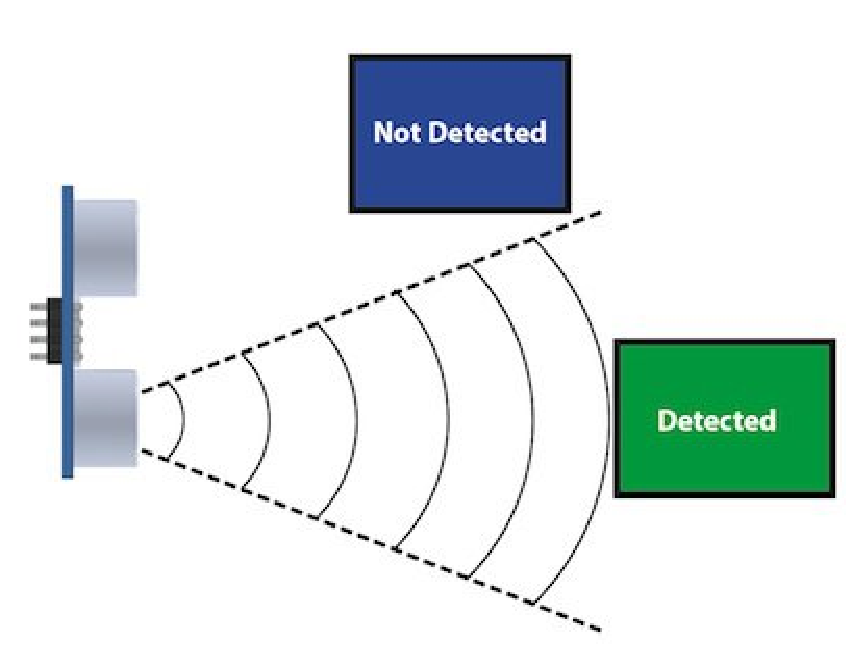
\includegraphics[scale=0.7]{figuras/cone2.eps}
    \caption{Emissão do Sinal Ultrasônico.}
    \label{img:conee}
  \end{figure}

  A partir da observação da Figura \ref{img:conee}, é possível identificar possíveis problemas gerados por esta característica. Basicamente,
  o sonar observa o ambiente de maneira unidimensional, em relação aos \textit{inputs} obtidos pelo mesmo. \textit{Inputs}, estes,
  que são compostos apenas da distância entre o robô e um objeto a sua frente. Entretando, estes \textit{inputs} são gerados a partir
  da iteração tridimensional do som com o ambiente, incluindo no resultado uma margem de erro importante, que não deve ser ignorada.

  Para analisar o impacto desta característica, deve-se compreender os detalhes técnicos do sonar utilizado, mais especificamente,
  a distância máxima de alcance do sonar e a angulação de emissão do sinal sonoro. Durante esta pesquisa, o
  sonar utilizado, presente no Kit Mindstorm NXT, possui uma angulação de emissão do sinal de 30 (trinta) graus e uma distância máxima de
  255 (duzentos e cinquenta e cinco) centímetros. Com estas informações é possível padronizar o ambiente e o contexto de utilização do sonar
  de uma forma que os resultados obtidos possuam uma margem de erro aceitável, de acordo com o contexto trabalhado.

  Com a emissão do sinal a uma angulação de 30 graus, por exemplo, obstáculos identificados a 180 centímetros podem possuir até 90
  centímetros de margem de erro, gerando um resultado pouco confiável para o contexto da Robótica Móvel. Desse modo, deve-se evitar
  a identificação de obstáculos a distâncias longas, as quais foram fixadas, durante esta pesquisa, em aproximadamente um metro de distância.

  Devido às características do sonar, a identificação de pontos de referência não se baseia em características físicas dos obstáculos,
  utilizando a relação de distância entre robô e obstáculo como forma de identificação de pontos de referência. A ideia não é
  identificar locais específicos que possuem pontos de referência, como a técnica da utilização de postes emissores de infra-vermelho,
  e sim a identificação da posição atual do robô em relação aos obstáculos, a qual viabiliza o processo de auto-localização do robô.

  Buscando a minimização da margem de erro, alguns detalhes do ambiente precisaram ser fixados, limitados e bem definidos. Foi fixado
  um tamanho máximo de 1,5 metros quadrados para o ambiente de navegação, assim como a utilização de obstáculos lisos e uniformes como
  pontos de referência. Basicamente, estes obstáculos se resumem a utilização de paredes na margem do ambiente de navegação, sem a utilização
  de obstáculos internos ao mapa.

  O sensor utilizado é o sonar original do Kit, o qual pode ser observado na Figura \ref{img:sonar_utilizado}.

  \begin{figure}[H]
    \centering
    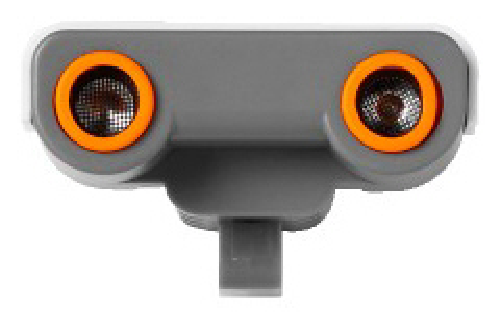
\includegraphics[scale=0.5]{figuras/ultrasonic.eps}
    \caption{Sensor de Distância Ultrasônico.}
    \label{img:sonar_utilizado}
  \end{figure}


\subsection{Colisões em Obstáculos}
\label{sub:colisao}

\section{Análise de Viabilidade}
\label{sec:viabilidade}
